\documentclass[oneside, 11pt]{article}

\usepackage[T1]{fontenc}
\usepackage[utf8]{inputenc}
\usepackage[dutch]{babel}

\usepackage{fouriernc}
\usepackage[detect-all, load-configurations=binary,
            separate-uncertainty=true, per-mode=symbol,
            retain-explicit-plus, range-phrase={ tot }]{siunitx}

\usepackage{setspace}
\setstretch{1.2}

\setlength{\parskip}{\smallskipamount}
\setlength{\parindent}{0pt}

\usepackage{geometry}
\geometry{marginparwidth=0.5cm, verbose, a4paper, tmargin=3cm, bmargin=3cm, lmargin=2cm, rmargin=2cm}

\usepackage{float}

\usepackage[fleqn]{amsmath}
\numberwithin{equation}{section}
\numberwithin{figure}{section}

\usepackage{graphicx}
\graphicspath{{Figures/}}
\usepackage{subfig}

\usepackage{tikz}
\usetikzlibrary{plotmarks}

\usepackage{fancyhdr}
\pagestyle{fancy}
\fancyhf{}
\rhead{\thepage}
\renewcommand{\footrulewidth}{0pt}
\renewcommand{\headrulewidth}{0pt}

\usepackage{relsize}
\usepackage{xspace}
\usepackage{url}

\newcommand{\figref}[1]{Figuur~\ref{#1}}

\newcommand{\hisparc}{\textsmaller{HiSPARC}\xspace}
\newcommand{\kascade}{\textsmaller{KASCADE}\xspace}
\newcommand{\sapphire}{\textsmaller{SAPPHiRE}\xspace}
\newcommand{\jsparc}{\textsmaller{jSparc}\xspace}
\newcommand{\hdf}{\textsmaller{HDF5}\xspace}
\newcommand{\aires}{\textsmaller{AIRES}\xspace}
\newcommand{\csv}{\textsmaller{CSV}\xspace}
\newcommand{\python}{\textsmaller{PYTHON}\xspace}
\newcommand{\corsika}{\textsmaller{CORSIKA}\xspace}
\newcommand{\labview}{\textsmaller{LabVIEW}\xspace}
\newcommand{\daq}{\textsmaller{DAQ}\xspace}
\newcommand{\adc}{\textsmaller{ADC}\xspace}
\newcommand{\adcs}{\textsmaller{ADC}s\xspace}
\newcommand{\Adcs}{A\textsmaller{DC}s\xspace}
\newcommand{\hi}{\textsc{h i}\xspace}
\newcommand{\hii}{\textsc{h ii}\xspace}
\newcommand{\mip}{\textsmaller{MIP}\xspace}
\newcommand{\hisparcii}{\textsmaller{HiSPARC II}\xspace}
\newcommand{\hisparciii}{\textsmaller{HiSPARC III}\xspace}
\newcommand{\pmt}{\textsmaller{PMT}\xspace}
\newcommand{\pmts}{\textsmaller{PMT}s\xspace}

\DeclareSIUnit{\electronvolt}{\ensuremath{\mathrm{e\!\!\:V}}}

\DeclareSIUnit{\unitsigma}{\ensuremath{\sigma}}
\DeclareSIUnit{\mip}{\textsmaller{MIP}}
\DeclareSIUnit{\adc}{\textsmaller{ADC}}

\DeclareSIUnit{\gauss}{G}
\DeclareSIUnit{\parsec}{pc}
\DeclareSIUnit{\year}{yr}



\title{Data retrieval}
\author{A.P.L.S. de Laat} 
\docanalyse{2}{DR}
\version{1.0}

\begin{document}

\maketitle

\section{Toegang tot \hisparc gegevens}

De data opslag van \hisparc meetgegevens op het \nikhef bestaat uit een
paar databases. Als eerst is er de ruwe dataopslag. Daarin worden
metingen opgeslagen zodra ze naar het \nikhef worden gestuurd. Daarnaast
is er nog een afgeleide database. In de afgeleide database zijn al een
aantal analyses op de meetgegevens uitgevoerd. Met name de aankomst
tijden van de shower in verschillende detectoren en het aantal deeltjes
in een detector.

Toegang tot \hisparc meetgegevens is vrij voor iedereen. Het downloaden
van de ruwe data is niet heel eenvoudig, bovendien raden we dat ook niet
meer aan nu de afgeleide database beschikbaar is. Data uit de afgeleide
database wordt als csv-bestand (tab gescheiden kolommen) aangeboden voor
download via deze website: \url{http://data.hisparc.nl/data/download}.

Zodra data gedownload is kan deze bijvoorbeeld in Excel geïmporteerd
worden om grafieken te maken en analyses uit te voeren. Omdat Excel niet
altijd even eenvoudig werkt hebben we zelf een programma gemaakt dat in
webbrowsers werkt. Het download data en kan daar direct grafieken mee
maken.


\section{\jsparc bibliotheek}

\jsparc is de JavaScript bibliotheek die het makkelijker maakt om met
\hisparc data te werken. Zo biedt de bibliotheek een eenvoudige functie
om gegevens op te halen van de \hisparc server en deze gelijk om te
zetten tot een formaat dat begrijpelijk is voor JavaScript.


\section{Data retrieval}

Dit is een beschrijving van de pagina te bereiken via
\url{http://data.hisparc.nl/media/jsparc/data_Retrieval.html}. Hiermee
kan data opgehaald en bestudeerd worden. Aan het \hisparc logo (rechts
boven) is te herkennen of de pagina data van de \hisparc server aan het
ophalen is, dan is het logo namelijk geanimeerd. Als eerst haalt de
pagina een up-to-date lijst van \hisparc stations op, dit gaat zo snel
dat het logo maar heel kort geanimeerd is.


\subsection{Downloading data}

Het Download data formulier staat men toe een \hisparc station, een
start- en einddatum, en het data type te selecteren. Door te drukken op
\emph{Get Data!} wordt de data dan gedownload. Zodra de nieuwe data is
geladen, verschijnt er een nieuwe sectie op de pagina die een overzicht
weergeeft van alle datasets die geladen zijn. Het is mogelijk meerdere
datasets te laden door het Download data formulier opnieuw te gebruiken
met andere instellingen. Met het rechter formulier; \emph{Load local
file} kan men eigen of eerder gedownloade .csv bestanden (tab
gescheiden) inladen. Deze verschijnen dan ook in het overzicht.

\begin{figure}
    \centering
    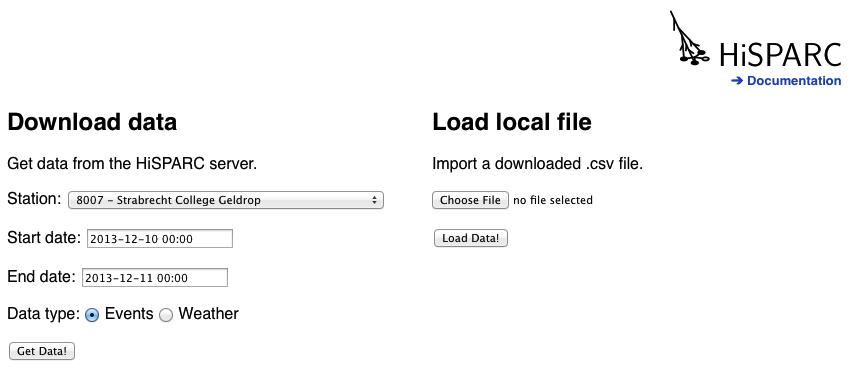
\includegraphics[scale=0.75]{get_data}
    \caption{Gedeelte van de website waar data mee gedownload of
             ingeladen kan worden.}
    \label{fig:get_data}
\end{figure}

\begin{figure}
    \centering
    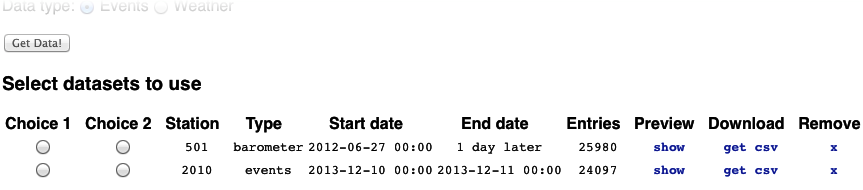
\includegraphics[scale=0.75]{data_overview}
    \caption{Overzicht van de ingeladen datasets.}
    \label{fig:get_data}
\end{figure}

Met de geladen datasets kunnen verschillende acties uitgevoerd worden.
Door in de \emph{Choice} kolommen een dataset te kiezen verschijnen de
plot opties en een lijst van de variabelen in die dataset. In sectie
\ref{subsec:plotting} is uitgelegd wat alle opties betekenen. Daarnaast
kan er gekozen worden om de waarden in de dataset te bekijken door op
\emph{show} te klikken in de \emph{Preview} kolom. Met de \emph{get csv}
knop wordt het .csv bestand gedownload. Met de \emph{x} in de
\emph{Remove} kolom kan de dataset uit het geheugen van de browser
gewist worden.


\subsection{Grafieken maken}\label{subsec:plotting}

Zodra een dataset gekozen is kunnen er plots (grafieken) mee gemaakt
worden. Er zijn 3 opties voor soorten grafieken. Bij het type
\emph{scatter} worden er twee variabelen voor iedere meting tegen elkaar
uitgezet, een op de x-as en de ander op de y-as. Bij het type
\emph{histogram} kan maar één variabele gekozen worden (x-as). Bij een
histogram wordt het hele bereik tussen de minimale en maximale waarde
van die variabele opgedeeld in een aantal (normaal 100) evengrote delen.
Dan wordt voor elke individuele waarde gekeken in welk bereik die past,
het aantal waarden in een bereik komt dan op de y-as te staan. Als
laatste is er nog de \emph{time series}. Hierbij is de x-as de tijd (en
datum) en kan een variabele voor de y-as gekozen worden.

Als de keuzes gemaakt zijn kan de plot gemaakt worden door op
\emph{Create Plot} te drukken. Als de opties aangepast worden kan een
nieuwe plot gemaakt worden door weer op die knop te drukken.

\begin{figure}
    \centering
    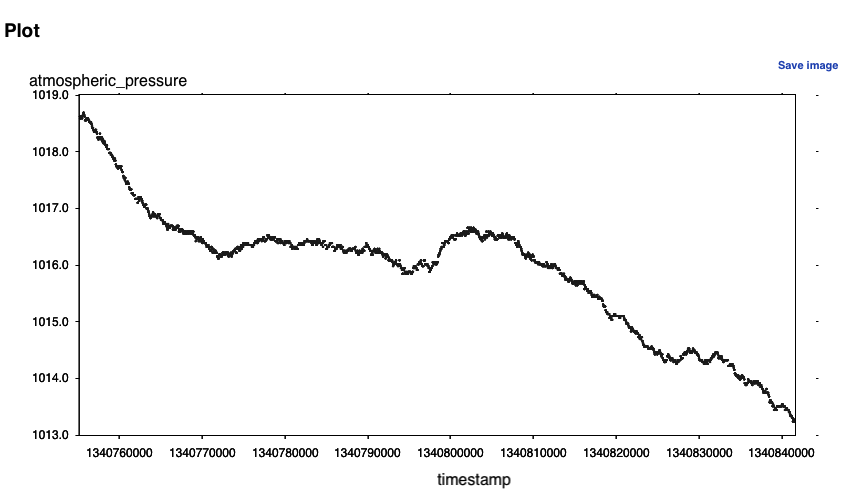
\includegraphics[scale=0.75]{plot}
    \caption{Voorbeeld van een plot. Hier is de luchtdruk op de y-as
             uitgezet tegen de tijdstempel op de x-as.}
    \label{fig:get_data}
\end{figure}


\subsection{Interpolatie}

Als meerdere datasets zijn opgehaald met overlappende tijdperiodes is
het mogelijk om deze tegen elkaar te plotten. Kies hiervoor een dataset
in kolom \emph{Choice 1} en de ander in \emph{Choice 2}. De variabelen
verschijnen dan naast elkaar zodat uit beide een keuze gemaakt kan
worden voor de x- en y-assen.


\begin{thebibliography}{9}
\end{thebibliography}

\end{document}
